\textbf{Липшициевость:}\\
Обозначение: $f\in C^{k, m}_L$. Пусть $m\leq k,\ L > 0$ -- константа Липшица, тогда:
$$f\in C^{k, m}_L \Leftrightarrow \left[
\begin{array}{ccc}
    & f\in C^k,                                                  \\
    & \|\nabla^mf(y)-\nabla^mf(x)\|\leq L\|y - x\|\ \forall x, y \\
\end{array}
\right.$$
В частности, если $f\in C^{1, 1}_L$, то верно

$$\|\nabla f(y)-\nabla f(x)\|\leq L\|y - x\|\ \  \Leftrightarrow\ \  \begin{array}{ccc}
                                                                         f(y) \leq f(x) + \nabla f(x)^T(y-x) + \dfrac{L}{2}\|y - x\|^2 \\
                                                                         f(y) \geq f(x) + \nabla f(x)^T(y-x) - \dfrac{L}{2}\|y - x\|^2
\end{array}
$$

\begin{figure}[H]
    \centering
    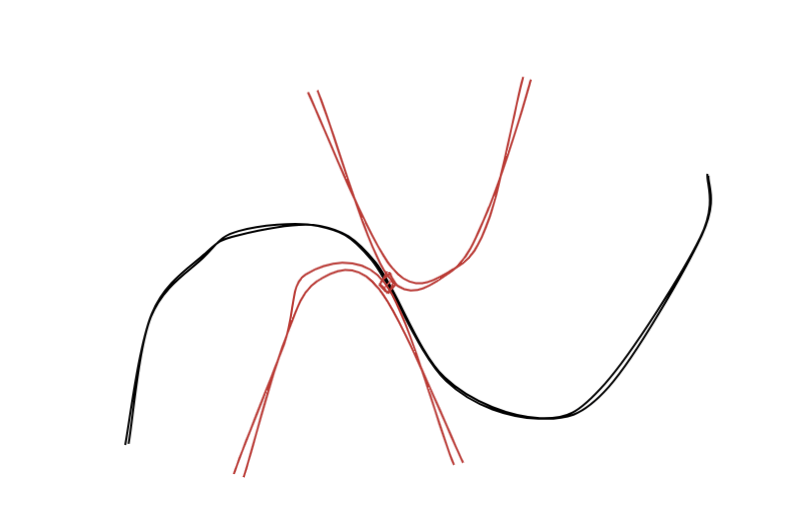
\includegraphics[width=0.5\textwidth]{images/lip.png}
    \caption{Липшициевость $f\in C^{1, 1}_L$ говорит о том, что в любой точке функцию сверху и снизу можно ограничить параболой, она не будет возрастать или убывать слишком быстро}
\end{figure}

А также можно сказать важные вещи про гессиан:
$$f\in C^{2, 1}_L\ \ \Leftrightarrow\ \ \nabla^2 f(x) \preccurlyeq LI\ \ \Leftrightarrow\ \ \lambda_{\max} (\nabla^2 f(x)) \leq L,$$

то есть максимальное собственное значение гессиана ограничено сверху константой Липшица.
В частности липшициевость означает, что не может быть вертиальных асимптот у функции.

\underline{Примеры}:
\begin{itemize}
    \item $f(x) = \sin(x)$ -- функция с липшициевым градиентом, так как $f\in C_L^{1, 1}$ и $|f'(y) - f'(x)| = |\cos(y) - \cos(x)| \leq L |x - y|$ с константой $L = 1$

    \item $f(x) = \exp(x)$ не является липшициевой, так как любые ее производные всегда будут возрастать экспоненциально.
\end{itemize}
\bigskip

\textbf{Выпуклость:}\\
\textbf{Определение.} Функция называется \textit{выпуклой}, когда $Dom(f)$ выпукла и $\forall x, y \in Dom(f)\   \forall \alpha \in [0; 1]$ верно, что

$$f(\alpha x + (1 - \alpha)y) \leq \alpha f(x) + (1 - \alpha) f(y).$$

В случае строгой выпуклости знак также строгий.\\
Для них верно следующее:

$$f(y) \geq f(x) + \nabla f(x)^T(y-x)\ \ \forall y, x$$

\begin{figure}[H]
    \centering
    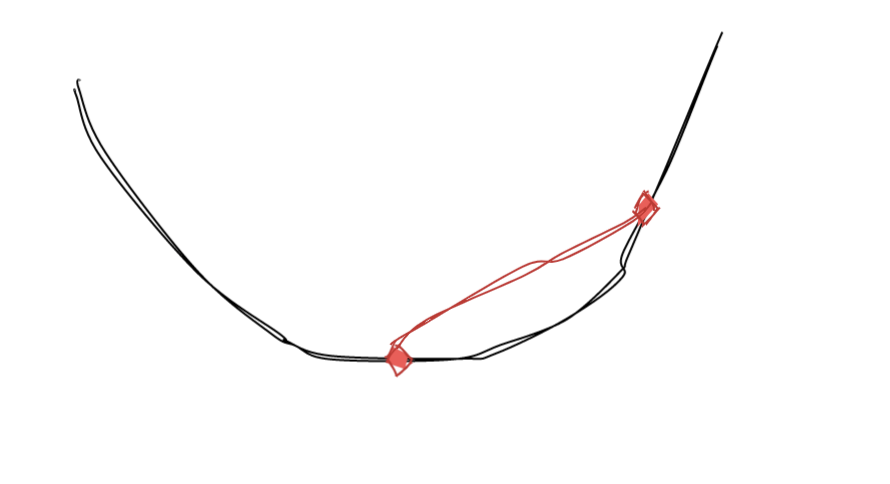
\includegraphics[width=0.5\textwidth]{images/conv.png}
    \caption{Выпуклость означает, что если между любыми двумя точками провести отрезок, функция окажется снизу}
\end{figure}

\underline{Примеры:}
\begin{itemize}
    \item $f(x) = x^2$ -- выпуклая
    \item $f(x) = \exp(x)$ -- выпуклая
    \item $f(x) = \log(x)$ не является выпуклой
\end{itemize}
\bigskip



\textbf{Сильная выпуклость.}

\textbf{Определение.} Функция называется \textit{сильно выпуклой} с параметром $\mu > 0$, если $f(x) - \dfrac{\mu}{2}\|x^2\|$ -- выпуклая.
Также справедливо:

$$f(x) - \dfrac{\mu}{2}\|x^2\|\text{ -- выпуклая} \Leftrightarrow f(y) \geq f(x) + \nabla f(x)^T(y-x) + \dfrac{\mu}{2}\|y-x\|^2\ \ \forall x, y$$

И еще:

$$f\in C^2, f - \mu\text{-сильно выпукла}\ \Leftrightarrow\ \lambda_{\min}(\nabla^2 f(x)) \geq \mu$$

Таким образом, если есть и липшициевость, и сильная выпуклость, максимальное и минимальное собственное значение гессиана ограничено, это круто.

\underline{Примеры:}
\begin{itemize}
    \item $f(x) = x^2$ -- сильно выпуклая с $\mu = 2$
    \item $f(x) = \exp(x)$ -- не является сильно выпуклой, т.к. вторя производная может быть сколь угодно близкой к 0
\end{itemize}